% !TeX root = ../documento.tex
\chapter{Introdução}
\label{cap:introducao}

Este capítulo apresenta uma visão geral do trabalho, descrevendo o contexto e os desafios que o motivaram (Seção~\ref{sec:contextualizacao} e Seção~\ref{sec:motivacao}). A partir disso, formaliza-se o problema de pesquisa (Seção~\ref{sec:definicao-do-problema}), as questões norteadoras (Seção~\ref{sec:questoes-de-pesquisa}) e as hipóteses elencadas (Seção~\ref{sec:hipoteses}). Por fim, são traçados os objetivos (Seção~\ref{sec:objetivos}), as contribuições esperadas (Seção~\ref{sec:contribuicoes}), as publicações decorrentes da pesquisa (Seção~\ref{sec:publicacao}) e a forma como o documento está estruturado (Seção~\ref{sec:organizacao}).

\section{Contextualização}
\label{sec:contextualizacao}

A convergência entre tecnologias de comunicação, eletrificação veicular e condução autônoma tem moldado um novo paradigma para o setor de transportes. O conceito de \gls{IoV} transforma veículos em sistemas computacionais sofisticados, capazes de viabilizar diversas aplicações de \gls{ITS}~\cite{RANI2023108543}. 

Veículos modernos são equipados com múltiplos sensores, unidades de processamento e interfaces de comunicação, permitindo a coleta e o processamento de grandes volumes de dados. Contudo, a complexidade das aplicações e a quantidade crescente de dados a serem processados podem exceder a capacidade computacional das \gls{OBU} instaladas.

Uma solução imediata seria aumentar a capacidade computacional dessas \glspl{OBU}, possibilitando maior processamento local. No entanto, o atual período de transição tecnológica resulta em cenários heterogêneos, no qual coexistem \glspl{OBU} com diferentes desempenhos~\cite{luo2024} e distintas tecnologias de comunicação~\cite{zheng2015}. Essa diversidade representa um desafio para a implementação de aplicações veiculares em larga escala, especialmente no contexto das cidades inteligentes (\textit{Smart Cities})~\cite{luo2024}.

Nesse ambiente fortemente dinâmico, muitas aplicações, em particular aquelas voltadas à condução autônoma, impõem requisitos rigorosos de latência~\cite{chao2025}. A execução integral do processamento nos dispositivos embarcados frequentemente inviabiliza o atendimento a tais requisitos, devido às limitações físicas de energia e desempenho~\cite{luo2024}.

Para superar essas restrições, destaca-se a \gls{VEC}, um paradigma onde servidores computacionalmente robustos são posicionados próximos aos veículos, reduzindo de forma significativa a latência de processamento~\cite{liu2021}. Tecnologias relacionadas, como a \gls{VCC}~\cite{whaiduzzaman2014} e a \gls{VFC}~\cite{keshari2022}, ampliam o escopo do processamento distribuído, oferecendo suporte adicional em diferentes níveis de proximidade e escalabilidade.

O descarregamento de tarefas surge como o mecanismo central para operacionalizar a comunicação e o processamento colaborativo entre veículos e essas arquiteturas distribuídas. Essa técnica consiste em migrar tarefas computacionais para nós mais capazes, como servidores de borda ou outros veículos com maior poder de processamento~\cite{wang2022}, possibilitando que dispositivos com recursos limitados executem aplicações veiculares complexas.

O principal desafio, entretanto, está em decidir quando e para onde descarregar as tarefas, considerando múltiplos fatores conflitantes, como tempo limite de processamento, custo energético, balanceamento de carga e qualidade do enlace de comunicação. Abordagens determinísticas, baseadas exclusivamente em heurísticas, apresentam desempenho limitado diante da alta variabilidade do ambiente veicular~\cite{ahmed2022}. Mobilidade intensa, flutuações do canal, sobrecarga de processamento e mudanças abruptas na carga computacional tornam as decisões estáticas rapidamente obsoletas, comprometendo a eficiência do sistema.

Essa limitação tem impulsionado a busca por soluções adaptativas e mais robustas, fundamentadas em aprendizado de máquina e sistemas inteligentes~\cite{mao2017,zhang2018,zhou2019,huang2020,shi2023,nieto2024}. Diante desse cenário, este trabalho visa propor uma arquitetura híbrida para o descarregamento de tarefas em redes \gls{VEC} que integra o ranqueamento multicritério Fuzzy-\gls{TOPSIS}~\cite{chen2000} com o \gls{DRL}. No entanto, como etapa intermediária e foco deste trabalho de qualificação, a solução foi inicialmente desenvolvida e avaliada utilizando o método \gls{TOPSIS} clássico~\cite{hwang1981}. Essa abordagem preliminar serviu para isolar e validar a eficácia da solução proposta.

% Neste sentido, nesta proposta, uma vez identificado o melhor candidato pelo \gls{TOPSIS}, o \gls{SAC} aprenderá uma política de decisão binária (descarregar ou executar localmente). Como extensão planejada, o \gls{TOPSIS} será substituído por \textit{\textit{Fuzzy}}-\gls{TOPSIS}~\cite{chen2000}, incorporando incerteza linguística aos critérios de avaliação dos candidatos.

% O \gls{TOPSIS} avalia três critérios de qualidade dos candidatos ao descarregamento: tempo de conclusão estimado (\gls{JCT}), consumo energético e distância ao nó de computação. Desta forma, a representação do ambiente veicular pelo agente de \gls{DRL} é reduzida, tornando-se mais compacta e com vetor de estado de dimensão fixa, o que contorna o problema da entrada variável nas redes neurais.



\section{Motivação}
\label{sec:motivacao}

A motivação para esta pesquisa fundamenta-se em três pilares críticos identificados após uma pesquisa bibliográfica no estado da arte das soluções de descarregamento de tarefas em redes veiculares.

Primeiramente, destaca-se a necessidade de viabilizar soluções de descarregamento em cenários onde coexistem veículos equipados com \gls{OBU} de capacidades computacionais e de comunicação distintas. Essa heterogeneidade exige modelos de decisão capazes de operar de forma eficiente independentemente das limitações do \textit{hardware} disponível e da tecnologia de acesso empregada~\cite{zheng2015, luo2024}.

Em segundo lugar, identifica-se uma lacuna de pesquisa relacionada à escalabilidade do \gls{DRL} em cenários veiculares dinâmicos. Isso ocorre porque os modelos de \gls{DRL} utilizam redes neurais que exigem um espaço de observação com tamanho fixo, fazendo com que a maioria das soluções existentes recorra a técnicas limitadas de representação do ambiente observado pelo agente ou exija o retreinamento sempre que a quantidade de nós candidatos ao processamento das tarefas varia~\cite{uddin2025,tang2024}. 

Por último, a realização de reengenharia de estado e de recompensa em \gls{DRL} é frequentemente descrita como um processo empírico e complexo devido à alta dimensionalidade e à falta de estruturação dos dados de entrada~\cite{shi2023}. 
Desenvolver uma abordagem que contorne essas limitações estruturais e que reduza a complexidade de decisão é um dos principais desafios abordados nesta proposta~\cite{ma2025}.

% Por último, a realização de reengenharia de estado e de recompensa em \gls{DRL} é frequentemente descrita como um processo empírico e complexo devido à alta dimensionalidade e à falta de estruturação dos dados de entrada~\cite{shi2023}. Esta pesquisa propõe mitigar esse problema ao utilizar o método de ranqueamento multicritério \textit{\textit{Fuzzy}}-\gls{TOPSIS}} como um facilitador da engenharia de estado, reduzindo a dimensionalidade e a complexidade da entrada da rede neural, facilitando o treinamento do modelo de \gls{DRL} para a tomada de decisão.

% Por fim, este trabalho de qualificação propõe uma abordagem evolutiva: inicialmente, emprega-se o \gls{TOPSIS} auxiliando o agente de decisão para validar a arquitetura proposta. Como etapa subsequente da pesquisa de doutorado, planeja-se a evolução para a lógica \textit{\textit{Fuzzy}}-\gls{TOPSIS}, visando incorporar a capacidade de lidar com a incerteza e a imprecisão inerentes aos cenários veiculares reais, aumentando a robustez do modelo final.

\section{Definição do Problema}
\label{sec:definicao-do-problema}

Diante das limitações de processamento local e da elevada variabilidade do ambiente veicular, o problema central investigado neste trabalho pode ser formulado da seguinte maneira:

\begin{quote}
\textbf{Como tomar decisões de descarregamento de tarefas, utilizando \gls{DRL}, em redes \gls{VEC}/\gls{V2X}, com número variável de candidatos ao processamento, não-estacionariedade, de forma confiável e adaptativa, cumprindo restrições de prazo e minimizando latência e consumo energético, sem necessidade de retreinamento diante de variações na densidade veicular?}
\end{quote}

Estudos recentes reforçam que a alta mobilidade veicular, a intermitência dos enlaces e a heterogeneidade de recursos computacionais tornam esse desafio ainda mais complexo~\cite{liu2021,mao2017,shi2023,nieto2024}. A decisão de descarregamento, em essência, configura-se como um problema de otimização \textit{NP-hard}~\cite{mao2017,feng2017}. Isso implica que soluções exatas em tempo polinomial são inviáveis, o que direciona a busca por métodos de baixa complexidade computacional e boa capacidade de adaptação. 

A literatura classifica as estratégias de decisão de descarregamento em três categorias principais: total (\textit{full offloading}), parcial (\textit{partial offloading}) e adaptativo (\textit{adaptive offloading})~\cite{wang2022}. A escolha entre essas abordagens impacta diretamente a formulação do problema e como a solução será estruturada.

\begin{figure}[ht!]
    \centering
    \Caption{\label{fig:offloading_categories} Formas de descarregamento de tarefas em \gls{VEC}: total (\textit{full offloading}), parcial (\textit{partial offloading}) e adaptativo (\textit{adaptive offloading}), com seus \textit{trade-offs} de confiabilidade e complexidade.}
    \UECEfig{}{
        \fbox{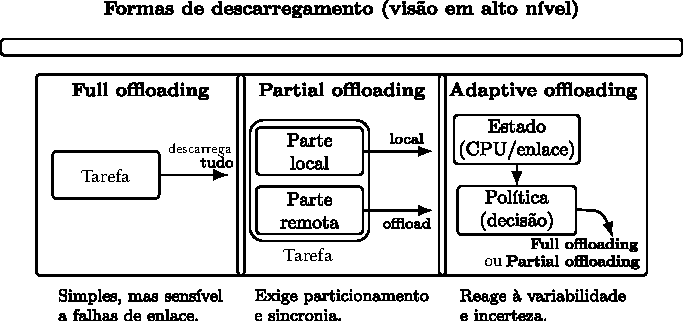
\includegraphics[width=12cm]{figuras/introducao/offloading_categories.pdf}}
    }{
        \Fonte{Elaborado pelo autor}
    }
\end{figure}

Como esquematizado na Figura~\ref{fig:offloading_categories}, o \textit{full offloading} consiste na transferência completa da tarefa da aplicação para um nó remoto, sendo uma estratégia de modelagem simplificada, porém extremamente sensível a falhas de comunicação e à latência da rede. O \textit{partial offloading}, por sua vez, divide a execução do programa entre os recursos locais do veículo e o servidor da rede veicular. Apesar de potencialmente reduzir a sobrecarga de transmissão e o tempo total de resposta, essa abordagem introduz o desafio do particionamento estrutural da tarefa e da sincronização de suas partes. Já o \textit{adaptive offloading} analisa dinamicamente o ambiente para decidir qual a estratégia é mais adequada para cada tarefa, entregando maior resiliência às custas de uma maior complexidade do modelo de tomada de decisão. 

Além disso, as estratégias de decisão variam entre abordagens que processam conjuntos de tarefas em lote (\textit{batch}) ou para cada tarefa, individualmente, direcionando a arquitetura das soluções propostas. A primeira abordagem é mais adequada para aplicações com cargas de trabalho previsíveis e tolerantes a atrasos, como transcodificação de vídeo e processamento de dados em massa~\cite{wang2022}. Nesses cenários, os algoritmos tendem a operar utilizando estatísticas globais para otimizar a alocação de recursos~\cite{li2020genetic, you2021efficient}. Contudo, por assumir parâmetros predeterminados e um ambiente estacionário, essa estratégia tem dificuldades em se adaptar a flutuações repentinas nos cenário observado~\cite{he2025, luo2024}. Em contrapartida, a segunda abordagem, focada na decisão reativa e individual por tarefa, é necessária para sistemas de tempo real e aplicações críticas, como condução autônoma e sensoriamento colaborativo~\cite{RANI2023108543}. Ao processar cada requisição no exato momento de sua chegada, o modelo consegue capturar a imprevisibilidade do ambiente e adaptar o descarregamento de forma contextualizada~\cite{uddin2025}. No entanto, essa abordagem possui uma elevada complexidade de otimização e alocação de recursos~\cite{kandali2025, zhao2025}.

% Avaliar instantaneamente o estado das filas, as restrições de canal e a disponibilidade de nós para cada tarefa isolada gera um severo gargalo computacional, o que justifica a adoção de algoritmos inteligentes e de rápida inferência, como o \gls{DRL}, capazes de balancear latência e energia sem comprometer a estabilidade operacional do sistema~\cite{miriyala2026, uddin2025}.

% Nesse contexto, aplicações com alta demanda computacional e baixa carga de dados (como visão computacional e algoritmos de navegação) impõem restrições de latência que superam a capacidade de processamento das \gls{OBU} locais. Para viabilizar tais aplicações, a tomada de decisão deve integrar, em tempo real, múltiplos indicadores conflitantes (latência, energia, carga de \gls{CPU} e qualidade do canal) sob forte incerteza de medição~\cite{liu2021}. 

Embora a literatura apresente métodos baseados em programação linear, algoritmos gulosos e meta-heurísticas~\cite{li2020genetic,you2021efficient}, tais abordagens operam principalmente sobre instantes isolados da rede (\textit{snapshots}) e assumem decisões de etapa única~\cite{xiang2025}. Essa forma de avaliar o problema pode limitar a eficácia dessas estratégias em cenários veiculares nos quais as métricas variam continuamente (não estacionariedade), pois elas não conseguem capturar o impacto a longo prazo das decisões sequenciais na qualidade de serviço percebida pelos usuários~\cite{uddin2025,cao2024survey}. Para que o descarregamento em redes \gls{V2I}/\gls{V2X} seja de fato confiável e adaptativo, é preciso modelar e lidar diretamente com a incerteza e a variabilidade do ambiente veicular.

Em contrapartida às abordagens tradicionais, as soluções baseadas em \gls{DRL} são capazes de otimizar recompensas sequenciais futuras. No entanto, enfrentam uma limitação estrutural severa, a dependência de um espaço de observação de tamanho fixo~\cite{uddin2025}. Para lidar com variações na quantidade de nós candidatos, a maioria dos modelos recorre a técnicas paliativas que comprometem a escalabilidade~\cite{miriyala2026}. Diante disso, evidencia-se a necessidade de investigar modelos híbridos. A integração de métodos de ranqueamento para filtrar e padronizar as entradas tem o potencial de aprimorar significativamente o processo decisório do \gls{DRL}, superando simultaneamente a inflexibilidade das heurísticas e as limitações estruturais das redes neurais~\cite{vieira2025}.

Adicionalmente, a tomada de decisão nesse ambiente ocorre sob condições de incerteza. Devido à intermitência dos enlaces e à alta latência na sinalização, as informações coletadas sobre a disponibilidade energética ou a carga de processamento dos vizinhos chegam frequentemente ruidosas ou desatualizadas aos agentes de decisão~\cite{uddin2025}. Essa imprecisão e a observabilidade parcial exigem uma avaliação de qualidade dos candidatos que considere a incerteza de forma explícita, buscando garantir a confiabilidade do descarregamento no mundo real~\cite{miriyala2026}. Sob essa ótica, a integração de técnicas que lidam com a incerteza linguística, como a lógica difusa, aos critérios de decisão se mostra promissora para mitigar a variabilidade dos parâmetros e aprimorar o desempenho da arquitetura de descarregamento~\cite{vieira2025, vemireddy2021}.

Outro fator importante diz respeito às tecnologias de comunicação e aos serviços de borda empregados no ambiente veicular. As tecnologias \gls{V2X} e \gls{V2I} viabilizam a troca de dados entre os veículos e a infraestrutura de forma eficiente e em tempo real. Nesse contexto, a arquitetura \gls{VEC} provê aos dispositivos veiculares uma plataforma distribuída para a execução de suas aplicações sensíveis à latência, operando sob a cobertura da rede celular \gls{5G} \gls{NR} para a comunicação com as infraestruturas de borda, e utilizando a interface de comunicação direta \gls{V2X} \textit{Sidelink} para a cooperação entre os veículos vizinhos~\cite{chao2025, luo2024}.


% Os principais desafios inerentes a esse ambiente são sintetizados na Figura~\ref{fig:problems}.

% \begin{figure}[ht!]
%     \centering
%     \Caption{\label{fig:problems}Principais problemas inerentes ao descarregamento de tarefas veicular: mobilidade e instabilidade do enlace, heterogeneidade de recursos e filas, custos energéticos, incerteza de medições, dependência de tecnologias/protocolos e complexidade \textit{NP-hard} sob restrições de latência e confiabilidade.}
%     \UECEfig{}{
%         \fbox{%
%         \resizebox{0.95\linewidth}{!}{%
%         \begin{tikzpicture}[
%           font=\scriptsize\sffamily,
%           node distance=7mm and 9mm,
%           >=Latex
%         ]
%           \tikzset{
%             box/.style={
%               draw, thick, rounded corners=2pt,
%               align=left, inner sep=4pt,
%               text width=3.4cm, minimum height=14mm
%             },
%             cbox/.style={
%               draw, thick, rounded corners=2pt,
%               align=center, inner sep=4pt,
%               text width=3.8cm, minimum height=14mm
%             },
%             arrow/.style={-Latex, thick},
%             group/.style={draw, thick, rounded corners=3pt, inner sep=6pt},
%           }

%           % -----------------------------
%           % Núcleo (centro)
%           % -----------------------------
%           \node[cbox] (decision) {\textbf{Decisão de descarregamento}\\local / MEC / V2V};

%           \node[cbox, above=of decision] (goals)
%             {\textbf{Objetivos / Restrições}\\
%              Reduzir tempo e energia.\\
%              Cumprir restrição de tempo das aplicações.\\
%              Balancear a carga entre os dispositivos.};

%           \node[cbox, above=of goals] (nphard)
%             {\textbf{Complexidade}\\
%              Otimização \textit{NP-hard}\\
%              Exige soluções rápida e adaptativas.};

%           \node[cbox, below=of decision] (model)
%             {\textbf{Modelagem e Protocolos}\\
%              5G NR / \gls{V2X}.\\
%              Descoberta/anúncio de recursos.\\
%              Protocolo para descarregamento.};

%           % -----------------------------
%           % Laterais (problemas do ambiente)
%           % -----------------------------
%           \node[box, left=of decision] (mob)
%             {\textbf{Mobilidade / Canal}\\
%              Flutuação do canal.\\
%              Intermitência na comunicaçao.};

%           \node[box, right=of decision] (hetero)
%             {\textbf{Recursos / Carga}\\
%              CPUs distintas.\\
%              Filas variáveis.\\
%              Balanceamento de carga.};

%           % Contexto acima das laterais (sem aumentar largura)
%           \node[box, above=of mob] (scen)
%             {\textbf{Cenário}\\
%              Urbano ou Rodoviário.\\
%              Densidade e tráfego distintos.};

%           \node[box, above=of hetero] (apps)
%             {\textbf{Aplicações}\\
%              Diferentes perfis e requisitos. 
%              Visão Computacional, Criptografia, Navegação etc.};

%           % Problemas inferiores
%           \node[box, below=of mob] (energy)
%             {\textbf{Energia}\\
%              Custo variável por ciclo.\\
%              Bateria / estado Energético.\\
%              Trade-off energia--tempo};

%           \node[box, below=of hetero] (unc)
%             {\textbf{Incerteza}\\
%              Medições ruidosas.\\
%              Estimativas imperfeitas.\\
%              Estado parcial.};

%           % -----------------------------
%           % Setas (sem cruzamentos)
%           % -----------------------------
%           \draw[arrow] (nphard) -- (goals);
%           \draw[arrow] (goals) -- (decision);

%           \draw[arrow] (model) -- (decision);

%           \draw[arrow] (mob) -- (decision);
%           \draw[arrow] (hetero) -- (decision);

%           \draw[arrow] (energy.north east) -- ($(decision.south west)+(2mm,0mm)$);
%           \draw[arrow] (unc.north west)   -- ($(decision.south east)+(-2mm,0mm)$);

%           \draw[arrow] (scen) -- (mob);
%           \draw[arrow] (apps) -- (hetero);

%           % Moldura (opcional)
%           \begin{pgfonlayer}{background}
%             \node[group, fit=(nphard)(goals)(decision)(model)(scen)(mob)(energy)(apps)(hetero)(unc)] {};
%           \end{pgfonlayer}

%         \end{tikzpicture}%
%         }%
%         }%
%     }{
%         \Fonte{Elaborado pelo autor}
%     }
% \end{figure}


\section{Questões de Pesquisa}
\label{sec:questoes-de-pesquisa}

Este trabalho busca responder às seguintes questões de pesquisa, formuladas a partir das limitações inerentes ao ambiente veicular, da complexidade do problema de descarregamento de tarefas e da necessidade de garantir confiabilidade, eficiência energética e baixa latência em sistemas \gls{VEC}/\gls{V2X}:

\begin{alineas}[label=QP\arabic*.]
    \item \textbf{Como realizar o descarregamento de tarefas em ambientes \gls{V2I}/\gls{V2X} de maneira confiável e adaptativa, considerando a alta variabilidade da mobilidade veicular, da carga computacional e da incerteza nas métricas de decisão?}

    \item \textbf{De que maneira o emprego de modelos híbridos baseados em \gls{DRL} pode aprimorar a qualidade das decisões de descarregamento de tarefas em cenários veiculares altamente dinâmicos, superando as limitações das abordagens determinísticas ou heurísticas?}

    \item \textbf{Em que medida a incorporação da incerteza linguística nos critérios de avaliação dos candidatos ao descarregamento, aprimora a tomada de decisão em cenários de alta mobilidade e informações imprecisas?}
\end{alineas}


\section{Hipóteses}
\label{sec:hipoteses}

A partir das questões acima e da fundamentação teórica apresentada, formulam-se as seguintes hipóteses de pesquisa:

\begin{alineas}[label=H\arabic*.]
    % Como realizar o descarregamento de tarefas em ambientes \gls{V2I}/\gls{V2X} de maneira confiável e adaptativa, considerando a alta variabilidade da mobilidade veicular, da carga computacional e da incerteza nas métricas de decisão?

    \item \textbf{O desenvolvimento de uma política de descarregamento de tarefas que represente o estado do sistema de forma invariante à escala e que considere a incerteza das métricas de decisão viabiliza a criação de um modelo com capacidade de generalização para diferentes cenários de mobilidade e carga de processamento.}

    % De que maneira o emprego de modelos híbridos baseados em \gls{DRL} pode aprimorar a qualidade das decisões de descarregamento de tarefas em cenários veiculares altamente dinâmicos, superando as limitações das abordagens determinísticas ou heurísticas?

    \item \textbf{O uso conjunto de técnicas de avaliação multicritério, focadas no estado imediato do sistema, e de modelos de aprendizado, voltados para a otimização de estados futuros, aprimora a qualidade e a adaptabilidade das decisões de descarregamento frente às limitações das abordagens estritamente determinísticas.}

    % Em que medida a incorporação da incerteza linguística nos critérios de avaliação dos candidatos ao descarregamento, aprimora a tomada de decisão em cenários de alta mobilidade e informações imprecisas?

    \item \textbf{A incorporação da lógica nebulosa nos critérios de avaliação dos candidatos ao descarregamento mitiga o impacto da imprecisão das informações coletadas, conferindo maior robustez e confiabilidade ao processo decisório em cenários de alta mobilidade e incerteza.}


\end{alineas}



\section{Objetivos}
\label{sec:objetivos}

A fim de formalizar o propósito desta pesquisa e as etapas necessárias para sua execução, esta seção detalha os objetivos pretendidos. As metas são apresentadas seguindo uma abordagem \textit{top-down}, partindo de uma visão consolidada da solução proposta até o detalhamento das etapas técnicas e de validação.

\subsection{Objetivo Geral}
\label{sec:objetivo-geral}

Este trabalho tem como objetivo geral desenvolver e avaliar um modelo híbrido de descarregamento de tarefas para redes \gls{VEC}/\gls{V2X}, capaz de garantir confiabilidade e adaptabilidade diante da mobilidade veicular, da variabilidade de carga e da imprecisão de métricas de rede. O modelo integrará métodos de ranqueamento multicritério a algoritmos de \gls{DRL}, gerando um processo decisório estruturado e invariante à escala. Como etapa intermediária, foco deste trabalho, propõe-se validar o acoplamento do ranqueamento multicritério determinístico com o agente de \gls{DRL}. A conclusão do trabalho prevê a extensão deste módulo para incorporar o tratamento de incerteza linguística aos critérios de decisão, culminando na validação da arquitetura completa em um ambiente de simulação.

\subsection{Objetivos Específicos}
\label{sec:objetivos-especificos}


\begin{alineas}[label=OE\arabic*.]
    \item \textbf{Investigar e revisar sistematicamente os modelos de descarregamento de tarefas em cenários \gls{VEC}, identificando as limitações das abordagens tradicionais e os desafios de escalabilidade e engenharia de estado no emprego do \gls{DRL}.}
    \item \textbf{Implementar e validar um módulo de ranqueamento multicritério responsável por pré-avaliar os nós candidatos, abstraindo a variabilidade do ambiente veicular e convertendo o espaço de observação em um vetor compacto, de dimensão fixa e normalizada (etapa intermediária do projeto).}
    \item \textbf{Desenvolver e avaliar uma política de decisão baseada em \gls{DRL} que, ao consumir o estado previamente estruturado pelo ranqueamento, consiga otimizar simultaneamente métricas conflitantes como latência, consumo energético e taxa de cumprimento de prazos (\textit{deadline}).}
    \item \textbf{Aprimorar o módulo de ranqueamento mediante a incorporação de técnicas de modelagem de incerteza (lógica difusa), com o intuito de tolerar ruídos e atrasos nas medições e conferir maior resiliência à etapa de filtragem dos nós candidatos.}
    \item \textbf{Integrar e validar a arquitetura híbrida completa em um simulador de redes de eventos discretos, com modelagem fidedigna de protocolos celulares e interfaces de comunicação veicular direta, conduzindo uma comparação sistemática de desempenho contra abordagens heurísticas e algoritmos do estado da arte.}
\end{alineas}

\section{Contribuições Esperadas}
\label{sec:contribuicoes}
Espera-se que este trabalho produza contribuições relevantes tanto do ponto de vista científico quanto do ponto de vista prático, sobretudo no contexto de sistemas veiculares inteligentes e computação de borda. As principais contribuições previstas são:

\begin{alineas}[label=CE\arabic*.]
\item \textbf{Proposição de uma arquitetura de decisão híbrida que acopla métodos de ranqueamento multicritério a um modelo de \gls{DRL}, demonstrando a capacidade de tomada de decisão adaptativa e de generalização estrutural para cenários com variadas densidades de tráfego veicular.}.

\item \textbf{Desenvolvimento e validação de módulos de ranqueamento que atuam simultaneamente como redutores de dimensionalidade do estado e como filtros de incerteza linguística, viabilizando o tratamento de informações ruidosas e atrasadas para aumentar a confiabilidade da seleção de nós candidatos.}.

\item \textbf{Construção e integração de modelos de avaliação em plataformas de simulação de rede, englobando aspectos realistas de mobilidade, heterogeneidade computacional e protocolos de comunicação celular e veicular direta (\textit{sidelink}), estabelecendo um ambiente fidedigno para testes de arquiteturas \gls{VEC}.}

\item \textbf{Avaliação extensiva e comparação sistemática do modelo híbrido proposto contra métodos heurísticos e abordagens puramente baseadas em \gls{DRL}, evidenciando os ganhos em métricas de desempenho críticas, tais como redução de latência, eficiência energética e taxa de atendimento a prazos (\textit{deadlines}).}

\item \textbf{Consolidação de um conjunto de diretrizes práticas para o projeto de sistemas de descarregamento em arquiteturas de borda veicular, orientando pesquisadores e engenheiros sobre a aplicação de métodos híbridos.}

\end{alineas}

\section{Publicação}
\label{sec:publicacao}

Como parte do desenvolvimento deste trabalho, foi submetido e aceito um artigo no periódico internacional \textit{Cluster Computing} (Springer), classificado como Q1 nas bases \textit{Scopus/SJR} e posicionado no percentil superior da área de \textit{Computer Networks and Communications}. O artigo, intitulado ``\textit{FOFF: an energy-efficient task offloading in VEC-enabled vehicular networks using fuzzy TOPSIS}''~\cite{vieira2025}, apresenta uma versão preliminar do modelo híbrido de descarregamento de tarefas proposto neste trabalho, incluindo a arquitetura conceitual e os primeiros resultados derivados de experimentos em simulação. A publicação serviu tanto como validação da relevância científica da abordagem quanto como etapa intermediária para o refinamento metodológico, a ampliação dos cenários simulados e o aprofundamento das análises apresentadas nos capítulos seguintes.

\section{Organização do Trabalho}
\label{sec:organizacao}

Este documento está estruturado partindo dos fundamentos teóricos até o delineamento da solução proposta e o planejamento para a finalização da pesquisa. A organização segue o seguinte formato:

\begin{itemize}
    % \item \textbf{Capítulo~\ref{cap:introducao} --- Introdução:} apresenta o contexto geral, a motivação, a definição do problema, as questões de pesquisa, hipóteses e objetivos, além das contribuições esperadas e publicações decorrentes.

    \item \textbf{Capítulo~\ref{cap:fundamentacao-teorica} --- Fundamentação Teórica:} discute os conceitos essenciais que sustentam este trabalho, abrangendo arquiteturas \gls{5G} \gls{NR} e \textit{Sidelink} \gls{V2X}, o paradigma de descarregamento de tarefas em ambientes \gls{VEC}, fundamentos de \gls{DRL} e o método de decisão multicritério \gls{TOPSIS} com sua extensão \textit{Fuzzy}-\gls{TOPSIS}.

    \item \textbf{Capítulo~\ref{cap:revisao-literatura} --- Revisão da Literatura:} realiza uma análise crítica de trabalhos recentes, explorando as principais técnicas e tendências voltadas ao descarregamento de tarefas em cenários veiculares altamente dinâmicos.

    \item \textbf{Capítulo~\ref{chap:proposta} --- Proposta:} detalha a arquitetura \gls{SAC}-\gls{TOPSIS} desenvolvida como etapa intermediária desta qualificação, descrevendo a integração entre o algoritmo Soft \textit{Actor}-\textit{Critic} e o ranqueamento multicritério, bem como a modelagem do ambiente de simulação e os resultados experimentais obtidos.

    \item \textbf{Capítulo~\ref{chap:conclusoes} --- Conclusão:} sintetiza as principais descobertas desta etapa de qualificação, discute as limitações atuais e aponta os próximos passos para a validação final do modelo.

    \item \textbf{Capítulo~\ref{cap:cronograma-pesquisa} --- Cronograma:} descreve o planejamento das atividades futuras para a conclusão do doutorado, estabelecendo os prazos para experimentos finais, redação da tese e defesa.

    \item \textbf{Apêndice~\ref{ap:conversao-alibaba} --- Conversão de Escala do \textit{Trace} Alibaba:} descreve o procedimento de conversão do \textit{trace} de carga de trabalho real do Alibaba para o contexto do cenário veicular simulado, detalhando os fatores de escala temporal adotados.
\end{itemize}